%\documentclass[12pt]{apa7}
\documentclass[man, noextraspace, floatsintext, 12pt]{apa7}
%\documentclass[12pt, noextraspace, floatsintext]{apa6}
%\documentclass[man, 12pt, noextraspace, floatsintext]{apa6}
%\documentclass[11pt]{article}

% ADD REVIEWING PACKAGE
\usepackage{easyReview}
% Show reviews/edits or not?
\setreviewson
%\setreviewsoff
% Line numbers for ease of pointing to lines
\usepackage{lineno} %[pagewise]
%\linenumbers

\usepackage{pdflscape}
%Math typesetting packages
\usepackage{amsfonts, amssymb, amsmath, latexsym, amsthm}
%for URLs in-text 
\usepackage{url}
% ================
% = Bibliography =
% ================
%APA style citations and references
%\usepackage[utf8]{inputenc}
%\usepackage{babel,csquotes,xpatch}
\usepackage[backend=biber, style=apa, natbib]{biblatex}
\addbibresource{references.bib}

%\usepackage[natbibapa]{apacite} 
% for hanging-indentation style using apacite
%\setlength{\bibindent}{2.5em}
%\setlength{\bibleftmargin}{0em}
% ==========
% = Floats =
% ==========
\usepackage{float}
% include external pictures
\usepackage{graphicx} %Graphics/figures
% rotate figures/tables
\usepackage{rotating} 
% For professional tables
\usepackage{booktabs,threeparttable, multirow} 
\usepackage{tabularx}
% For fixing the column widths
\usepackage{array}
\newcolumntype{L}[1]{>{\raggedright\let\newline\\\arraybackslash\hspace{0pt}}m{#1}}
\newcolumntype{C}[1]{>{\centering\let\newline\\\arraybackslash\hspace{0pt}}m{#1}}
\newcolumntype{R}[1]{>{\raggedleft\let\newline\\\arraybackslash\hspace{0pt}}m{#1}}

% ===================
% ==== Tikz Diagrams	==
% ===================
\usepackage{tikz}
\usetikzlibrary{calc,arrows,positioning,shapes,shapes.gates.logic.US,trees, intersections}
% =======================
% === Other useful packages ==
% =======================
\usepackage[T1]{fontenc} 
\usepackage{placeins}
\usepackage{hyperref}
% subcaptions/subfigures %,justification=centered
\usepackage[hypcap=true,width=\textwidth]{subcaption}
% =============
%  == formatting ==
% =============
% \usepackage[margin=1in]{geometry}
% \setlength{\parindent}{0.5in}
\usepackage{setspace}
% \doublespacing

% ==========
% = Syntax =
% ==========
% For Computer Code in Appendix. I set the language for R, so will need to be changed for different languages
\usepackage{listings}
\lstset{
    language=R,
    basicstyle=\small \ttfamily,
    commentstyle=\ttfamily ,
    showspaces=false,
    showstringspaces=false,
    showtabs=false,
    frame=none,
    tabsize=2,
    captionpos=b,
    breaklines=true,
    breakatwhitespace=false,
    title=\lstname,
    aboveskip=10pt,
    belowskip=-10pt,
    %escapeinside={},
    %keywordstyle={},
   % morekeywords={}
    }%
%~~

\title{Multilevel latent transition analysis for organizational research}
\shorttitle{Multilevel Latent Transition Analysis} % For APA package

%\author{REMOVED FOR PEER REVIEW}
%\affiliation{REMOVED FOR PEER REVIEW}
\author{Grant B. Morgan \\ Kevin E. Wells \\ R. Noah Padgett}
\affiliation{Baylor University}

\abstract{
%\singlespacing
Person-centered methodologies generally refer to those that take unobserved heterogeneity of populations into account. The use of person-centered methodologies has proliferated, which is likely due to a number of factors, such as methodological advances coupled with increased personal computing power and ease of software use. The purpose of the proposed paper is to (1) present and discuss multilevel latent transition analysis and considerations for its use and (2) conduct a simulation study to assist researchers with both how to use measures of model-data fit and when to use them, and (3) demonstrate variance decomposition. With respect to the model parameters, the estimates tended to be unbiased, on average, but were prone to considerable variability. The standard errors were consistently over- or under-estimated and should not likely be trusted/interpreted. The problems with the standard errors naturally affects the confidence one might have in her parameter estimates in a negative way. Additional simulation will be necessary to find the boundaries of where the standard error estimation via the built-in algorithm can be trusted.Ultimately, we cannot yet recommend use of these models within the conditions that were simulated in this study.
} % End abstract

\keywords{Multilevel LTA}

%\authornote{REMOVED FOR PEER REVIEW}
\authornote{
Grant B. Morgan, Department of Educational Psychology, Baylor University; Kevin Wells, Department, University; R. Noah Padgett, Department of Educational Psychology, Baylor University.

%This research using data from R. Noah Padgett's master's thesis on fit in multilevel CFA models.
%This research was supported by Baylor University and the Department of Educational Psychology as funding toward the completion of my doctoral degree. 

%Acknowledgments\\ 
%I would like to thank the Grant Morgan, Nicholas Benson and  Mandy Hering for their efforts help in reviewing this project when it was R. Noah Padgett's Master's Thesis project.
%And thanks to Grace Aquino from the Baylor's Graduate Writing Center for her helpful feedback and editing.

Correspondence concerning this article should be address to Grant B. Morgan, Department of Educational Psychology, One Bear Place \# 97304, Baylor University, Waco, TX 76798. Contact: \href{mailto:grant\_morgan@baylor.edu}{\tt grant\_morgan@baylor.edu} 
}


\begin{document}

\maketitle

%% Spacing for Eqations Can't be in preamble...
\setlength{\abovedisplayskip}{3pt}
\setlength{\belowdisplayskip}{3pt}

Review of papers with multilevel LTA 





Efforts to classify individual cases into homogeneous groups have long been used in order to better understand complex sets of information. Classification of cases into homogeneous groups has important implications in the social sciences, such as education, medicine, psychology, or economics, where identifying smaller subsets of like cases may be of particular interest.  Person-centered methodologies generally refer to those that take unobserved heterogeneity of populations into account. That is, rather than treat all individuals as if they originated from a single underlying population, as is true with variable-centered methodologies  person-centered methodologies allow for multiple subpopulations to underlie a set of data. The challenge with these methods is identifying the correct number (i.e., frequency) of subpopulations, or classes, and the parameters (i.e., form) associated with each, when the frequency and form are not known \textit{a priori}. Although, multilevel mixture models are available to researchers, they have not been methodologically examined or discussed as extensively as other cross-sectional and longitudinal \textit{mixture} models. 

\subsection*{Introduction to Multilevel Latent Transition Analysis}
Using latent class analysis and its extension for longitudinal data, (latent transition analysis [LTA]), multiple underlying, homogeneous subgroups can be inferred from a set of categorical and/or continuous observed variables within a large heterogeneous data set. Such analyses allow researchers to statistically treat members of different subgroups separately, which may provide researchers with more power to detect effects of interest and closer alignment between statistical modeling and one's guiding theory. Furthermore, the hierarchical structure of organizational data must also be taken into account; that is, students (i.e., level-1 units) are nested within teacher/schools (i.e., level-2 units). Finally, multilevel LTA can be used to estimate the number of classes in each structured unit and the potential movement, or transitions, participants make between classes across time. The transitions/stability between latent classes across time can be treated as the outcome in and of itself, or the transitions/stability can be used as a correlate or predictor of some other, distal outcome.

From \citet{Asparouhov2008}, the multinomial logistic regression for the latent classification variable at time 1, $C_1$, can be expressed:

\begin{equation}
\textrm{P}(C_{1ij}=c)=\frac{\exp(\alpha_{1cj}+\boldsymbol{\beta}_{1cj}x_{1ij})}{\sum_c \exp(\alpha_{1cj}+\boldsymbol{\beta}_{1cj}x_{1ij})}
\end{equation}

The multinomial logistic regression for the latent classification variable at time 2 using $C_1$ as a covariate can be expressed:

\begin{equation}
\textrm{P}(C_{2ij}=d \vert C_{1ij}=c)=\frac{\exp(\alpha_{2dj}+\gamma_{dcj}+\boldsymbol{\beta}_{2dj}x_{2ij})}{\sum_d \exp(\alpha_{2dj}+ \gamma_{dcj} +\boldsymbol{\beta}_{2dj}x_{2ij})}
\end{equation}

The simplest case in which there are two data collection points is shown in \autoref{fig:pathModel-MLTA}.  The decomposition of variance for this model (i.e., proportion of variance in $C_2$ explained by the model) can be conducted in 11 steps.



\begin{figure}[ht]
\centering
\scriptsize
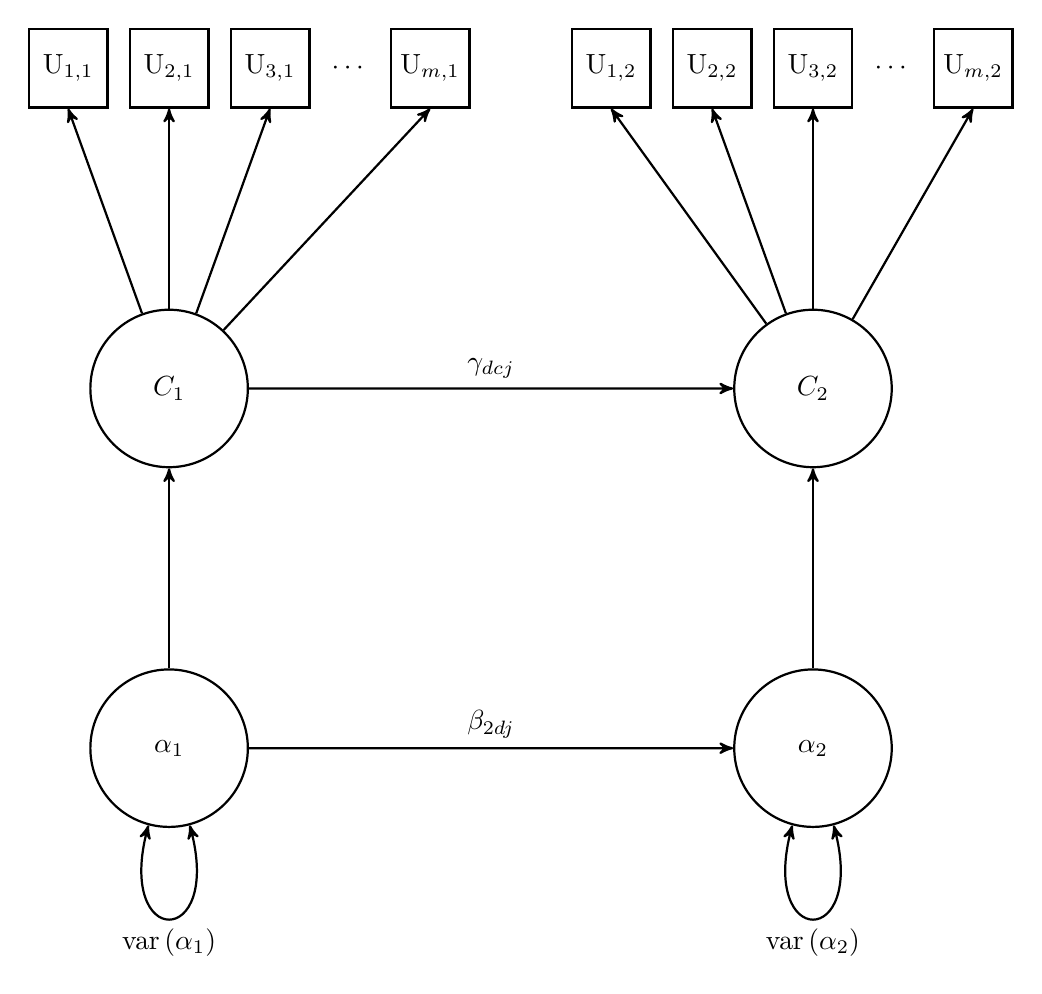
\begin{tikzpicture}[auto,scale=2,
	latent/.style={circle,draw,thick,inner sep=0pt,minimum size=20mm},
	error/.style={circle,inner sep=0pt,minimum size=10mm},
	manifest/.style={rectangle,draw,thick,inner sep=0pt,minimum size=10mm},
	corr/.style={<->,>=stealth', bend right=30},
	intercept/.style={regular polygon,
        regular polygon sides=3,draw,thick,inner sep=0pt,minimum size=10mm},
	mean/.style={regular polygon,regular polygon sides=3,draw,thick,inner sep=0pt,minimum size=20mm},
	paths/.style={->, thick, >=stealth'},
	variance/.style={<->, thick, >=stealth', bend left=270},
	varianceTop/.style={<->, thick, >=stealth', bend right=270, looseness=2},
	unique/.style={<->, thick, >=stealth', loop above=270, looseness=8},
	factvar/.style={<->, thick, >=stealth', loop below=90, looseness=8},
	ghost/.style={rectangle,draw,thick,inner sep=0pt,minimum size=0mm},
	dots/.style={rectangle,draw,thick,inner sep=0pt,minimum size=2mm, color=white, text=black}
	]
\tikzset{mystyle/.style={->,double=black}} 
\node [latent] (c1) {$C_1$};


\node [manifest] (u2)  [above = 1in of c1] {$\textrm{U}_{2,1}$};
\node [manifest] (u1)  [left = .1in of u2]  {$\textrm{U}_{1,1}$};
\node [manifest] (u3)  [right = .1in of u2]  {$\textrm{U}_{3,1}$};
\node [dots] (dots1)  [right = .1in of u3]  {$\cdots$};
\node [manifest] (u4)  [right = .1in of dots1]  {$\textrm{U}_{m,1}$};

\node [manifest] (u5)  [right = .5in of u4]  {$\textrm{U}_{1,2}$};
\node [manifest] (u6)  [right = .1in of u5] {$\textrm{U}_{2,2}$};
\node [manifest] (u7)  [right = .1in of u6]  {$\textrm{U}_{3,2}$};
\node [dots] (dots2)  [right = .1in of u7]  {$\cdots$};
\node [manifest] (u8)  [right = .1in of dots2]  {$\textrm{U}_{m,2}$};

\node [latent] (c2) [below = 1in of u7] {$C_2$};

\node [latent] (a1) [below = 1in of c1] {$\alpha_1$};
\node [latent] (a2) [below = 1in of c2] {$\alpha_2$};

\draw [paths] (c1) to node {} (u1.south);
\draw [paths] (c1) to node {} (u2.south);
\draw [paths] (c1) to node {} (u3.south);
\draw [paths] (c1) to node {} (u4.south);
\draw [paths] (c2) to node {} (u5.south);
\draw [paths] (c2) to node {} (u6.south);
\draw [paths] (c2) to node {} (u7.south);
\draw [paths] (c2) to node {} (u8.south);

\draw [paths] (c1) to node {$\gamma_{dcj}$} (c2.west);
\draw [paths] (a1) to node {$\beta_{2dj}$} (a2.west);
\draw [paths] (a1) to node {} (c1.south);
\draw [paths] (a2) to node {} (c2.south);

\draw [factvar] (a1) to node {$\textrm{var}\left(\alpha_1\right)$} (a1);
\draw [factvar] (a2) to node {$\textrm{var}\left(\alpha_2\right)$} (a2);
\end{tikzpicture}
\caption{Conceptual diagram of a multilevel latent transition model with two time points and $m$ latent class indicators at each time point.}\label{fig:pathModel-MLTA}
\end{figure}

\subsection*{Variance Decomposition}
Ultimately, these models tend to focus on explaining latent class membership at time 2. 
Latent class membership at time 2 is affected by $\alpha_1$, $C_1$, and $\alpha2$ so the variability of latent class membership at time 2 has to be carefully decomposed using a series of steps. 
The parameters chosen for simulation produced models that accounted for between 9.8\% and 62.9\% of the variability in latent class membership at time 2. 
Below we demonstrate the variance decomposition for the model that explained the maximum variability in latent class membership at time 2. 
For ease of explanation, we refer to latent class membership at times 1 and 2 as $C_1$ and $C_2$, respectively, and  the level-2 variance at times 1 and 2 as $\alpha_1$ and $\alpha_2$, respectively. 
We use the terms schools to refer to level-2 units and students to refer to level-1 units.

\begin{enumerate}
\item Proportion of variability in $C_1$ by $\alpha_1$.

The proportion of variability in $C_1$ explained by $\alpha_1$ is the same as the ICC for a multilevel logistic model. 

\[ ICC = \frac{\textrm{var}(\alpha_1)}{\textrm{var}(\alpha_1) + \frac{\pi^2}{3}} = \frac{2}{2 + 3.29} = .378\]

The parameter estimate itself ($\textrm{var}(\alpha_1)=2$) suggests the the proportion of students in classes 1 and 2 at time 1 varies depending on the school. In other words, class 1 contains about 50\% of the students at time 1 on average, but this percentage may differ across schools. The larger the parameter estimate, the greater the school effect. 

\item Find the variance of $C_1$. 

The proportion of students in each latent class at time 1 in the population is .5. Thus, the variance of $C_1$ is:
\[ \textrm{var(C}_1)=.50\times(1-.50) = .25 \]

\item Find the total contribution of $C_1$ on $C_2$.
\[ \gamma^2\times\textrm{var(C}_1)=3.5^2\times.25 = 3.06 \]

\item Split the contribution of $C_1$ on $C_2$ based on the proportion explained by $\alpha_1$:
\[ 3.06\times.378 = 1.16\]
and the residual of $C_1$:
\[ 3.06 \times (1-.378) = 1.90 \]

\item Next, we need to determine the contribution of $\alpha_1$ to $C_2$; $\alpha_1$ affects $C_2$ through $C_1$ and $\alpha_2$. The contribution of $\alpha_1$ on $C_2$ via $\alpha_2$ is:
\[ \beta^2\times\textrm{var}(\alpha_1)=.5^2\times2 = .5\]
The total contribution of $\alpha_1$ is:
\[ 1.16 + .5 +2\sqrt{.1.16\times.5}=3.18\]

\item Find the total variance of $C_2$ by adding the individual contributions.
\[ \textrm{level-1 residual} + 1.16 + 3.18 + \textrm{var(C}_2) = 3.29 + 1.16+ 3.18 + 0.5 = 8.87 \]

\item Compute the proportion of variance in $C_2$ explained by $\alpha_1$.
\[ \frac{3.18}{8.87} = .358 \]

\item Compute the proportion of variance in $C_2$ explained by residual variance of $\alpha_2$.
\[ \frac{0.5}{8.87} = .06 \]

\item Compute the proportion of variance in $C_2$ explained by residual of $C_1$.
\[ \frac{1.90}{8.87} = .215 \]

\item Find total proportion of variance in $C_2$ explained by the model.
\[ .358 + .06 + .215 = .629 \]

\item Find total proportion of variance in $C_2$ explained by $C_1$.
\[ \frac{3.06}{8.87}=.345 \]

\item Find the additional proportion of variance in $C_2$ by adding the school-level effect at time 2.
\[ .629 - .345 = .284 \]

\end{enumerate}
A similar decomposition is possible for higher number of latent classes at each timepoint.
However, the decomposition is more involved given the complexity of more transitions and random effects at level-2.
In our supplemental material, we have demonstrated this decomposition using the simulated three-class model described later.


\subsection*{Statement of Purpose}
Due to a number of programming constraints, systematic methodological investigations of multilevel LTA have not been conducted, which poses a problem for applied analysts. That is, little is known about the accuracy with which parameters are estimated in these models under virtually any real world conditions. The purpose of this paper is address this gap in the literature and knowledge base by employing Monte Carlo methods to examine the parameter accuracy under known conditions. In addition to providing the model output and interpretations, we also explain the variance decomposition, which is more complex than in traditional hierarchical linear models.

\section*{Methods}
The population structure used in the proposed study is a mixture model with known number of latent classes, class prevalence, and class-specific indicator distributions. The population structure also includes local independence. Models will then be estimated to determine the extent to which the true structure was recovered.  Mplus was used to generate all data and estimate each model. 

\subsubsection*{Design Factors}
We manipulated four factors in this study -- the level-2 variance at time 2, the transition between latent classes at time 1 and time 2, the effect of the level-2 unit across time, and the sample sizes. The level-2 variances at time 2 were 0.0, 0.25, or 0.5. The transition effect of latent class membership at time 1 on latent class membership at time 2 was 1, 2, or 3.5 (in odds ratio units). The effect of the level-2 units across time was 0.1, 0.3, or 0.5. The overall sample size was 500 or 1,000 but were based on different combinations of level-2 and level-1 units. That is, the level-2/level-1 within level-2 sample sizes were 50/10, 25/20, 100/5, and 50/20. All factors were fully crossed, which produced 108 (3 level-2 variances $\times$ 3 transition parameters $\times$ 3 level-2 effects $\times$ 4 sample sizes= 108) cells in the design. Each cell was replicated 100 times. The design factors and their associated levels are shown in \autoref{fig:designfactors}.


\begin{figure}[ht]
\centering
\scriptsize
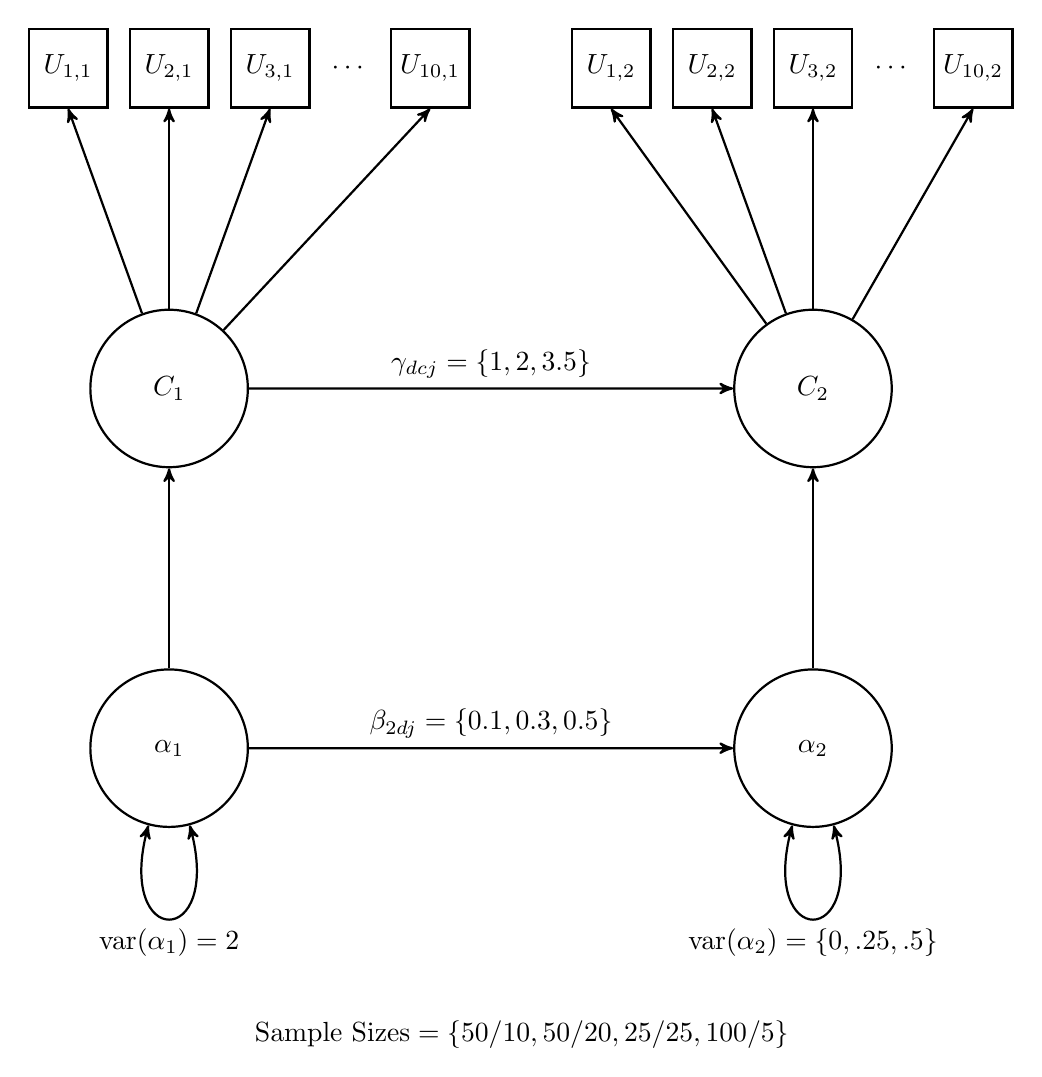
\begin{tikzpicture}[auto,scale=2,
	latent/.style={circle,draw,thick,inner sep=0pt,minimum size=20mm},
	error/.style={circle,inner sep=0pt,minimum size=10mm},
	manifest/.style={rectangle,draw,thick,inner sep=0pt,minimum size=10mm},
	corr/.style={<->,>=stealth', bend right=30},
	intercept/.style={regular polygon,
        regular polygon sides=3,draw,thick,inner sep=0pt,minimum size=10mm},
	mean/.style={regular polygon,regular polygon sides=3,draw,thick,inner sep=0pt,minimum size=20mm},
	paths/.style={->, thick, >=stealth'},
	variance/.style={<->, thick, >=stealth', bend left=270},
	varianceTop/.style={<->, thick, >=stealth', bend right=270, looseness=2},
	unique/.style={<->, thick, >=stealth', loop above=270, looseness=8},
	factvar/.style={<->, thick, >=stealth', loop below=90, looseness=8},
	ghost/.style={rectangle,draw,thick,inner sep=0pt,minimum size=0mm},
	dots/.style={rectangle,draw,thick,inner sep=0pt,minimum size=2mm, color=white, text=black}
	]
\tikzset{mystyle/.style={->,double=black}} 
\node[latent](c1) {$C_1$};

\node[manifest] (u2) [above = 1in of c1] {$U_{2,1}$};
\node[manifest](u1) [left = .1in of u2] {$U_{1,1}$};
\node[manifest](u3) [right = .1in of u2] {$U_{3,1}$};
\node[dots](dots1) [right = .1in of u3] {$\cdots$};
\node[manifest](u4) [right = .1in of dots1] {$U_{10,1}$};

\node[manifest](u5) [right = .5in of u4] {$U_{1,2}$};
\node[manifest](u6) [right = .1in of u5] {$U_{2,2}$};
\node[manifest](u7) [right = .1in of u6] {$U_{3,2}$};
\node[dots](dots2) [right = .1in of u7] {$\cdots$};
\node[manifest](u8) [right = .1in of dots2] {$U_{10,2}$};

\node[latent](c2)[below = 1in of u7] {$C_2$};

\node[latent](a1)[below = 1in of c1]{$\alpha_1$};
\node[latent](a2)[below = 1in of c2]{$\alpha_2$};

\draw[paths](c1) to node{}(u1.south);
\draw[paths](c1) to node{}(u2.south);
\draw[paths](c1) to node{}(u3.south);
\draw[paths](c1) to node{}(u4.south);

\draw[paths](c2) to node{}(u5.south);
\draw[paths](c2) to node{}(u6.south);
\draw[paths](c2) to node{}(u7.south);
\draw[paths](c2) to node{}(u8.south);

\draw[paths](c1) to node{$\gamma_{dcj}=\{1, 2, 3.5\}$}(c2.west);
\draw[paths](a1) to node{$\beta_{2dj}=\{0.1, 0.3, 0.5\}$}(a2.west);

\draw[paths](a1) to node{}(c1.south);
\draw[paths](a2) to node{}(c2.south);

\draw[factvar](a1) to node{$\textrm{var}(\alpha_1)=2$}(a1);
\draw[factvar](a2) to node{$\textrm{var}(\alpha_2)=\{0, .25,.5  \}$}(a2);

\node[ghost](shh) [right = .25in of u4] {};
\node[dots](blank)[below = 4.75in of shh] {$\textrm{Sample Sizes}=\{50/10,50/20,25/25,100/5 \}$};
\end{tikzpicture}
\caption{Path diagram of a multilevel latent transition model with manipulated levels of design factors.}\label{fig:designfactors}
\end{figure}

Each simulated model 10 latent class indicators at times 1 and 2, and class enumeration was limited to two. The latent class prevalence used for the two class population models was .50-.50 at time 1. Classes will be separated based on class-specific response probabilities to the dichotomous class indicators. 


\subsection{Parameter Values in Literature}

In the applications I have read so far, VERY few have fully reported the parameters of the model.

For the different parameters, I have pieces references together to help justify the different pieces.

 
\subsubsection{Transition Structure}

Here, there are two we will focus on

1. Unstructured 2 class model
Auerbach and collins (2006)
Vermunt (2010) 4.5.2

Crayen et al. (2012) - unstructured

\citep{Asparouhov2008}
low transition in from 1 to 2
higher transition from 2 to 1

\begin{table}[!htp]
\centering
\begin{threeparttable}
\caption{Two-class MLTA generating model details}
\label{tb:model-1}
\begin{tabular}{l r c r r r }
\toprule
& & & \multicolumn{3}{c}{Transition Matrix}\\ \cmidrule(lr){4-6}
\multicolumn{2}{l}{Class Size ($T=1$)} & & $C_{(t-1)\setminus t}$ & $C_2 =1$ & $C_2 =2$   \\ \midrule
\multicolumn{6}{c}{Probability Scale}\\
0.4	&  & &  $C_1 =1$	& 0.80  & 0.20  \\
0.6	&  & &  $C_1 =2$	& 0.07  & 0.93 \\
\multicolumn{6}{c}{Logit Parameterization}\\
$-0.405$	&  & & $C_1 =1$	& $1.37$    & 0\tnote{a}\\
0\tnote{a}	&  & & $C_1 =2$	& $-2.62$  & 0\tnote{a} \\ \midrule
\multicolumn{3}{l}{Random Effects} & \multicolumn{3}{r}{Regression Weights}\\ 
\multicolumn{3}{l}{$\mathrm{var}(\alpha_1) = \left\lbrace 0.8, 2.5\right\rbrace$} & \multicolumn{3}{r}{$\gamma = 4$}\\ 
\multicolumn{3}{l}{$\mathrm{var}(\alpha_2) = \left\lbrace 0.0, 0.25\right\rbrace$} & \multicolumn{3}{r}{$\beta = 0.3$}\\
 \bottomrule
\end{tabular}
 \vspace*{1mm}
 	\begin{tablenotes}[para, flushleft]
    {\small
        \textit{Note.} Parameters in brackets define the different values used as design factors. $\rm ^{a}$parameter fixed for identification.
    }
 	\end{tablenotes}
 \end{threeparttable}
\end{table}


Next, compute the different $R^2$ statistics to show how they change w.r.t. the variance components.

\textbf{Stage-sequential 3-class model}.
In the next model simulated, used a stage-sequential model with three classes.
The
"longitudinal Guttman  process", Piaget's (1947,; 1971) stages of cognitive development.

Piaget, J. (1947). Psychologie der intelligez [The psychology of intelligence]. Zurich, Switzerland: Rascher.
Piaget, J. (1971). The theory of stages in cognitive development. In R. D. Green, M. P. Ford, \& G. B. Flammer (Eds.), Measurement and Piaget (pp. 1–11). New York: McGraw-Hill.


Kolberg's (1980) stages of moral development

Collins (2002) exploration with substance abuse in youth

Reading development (kaplan)

\citep{Kaplan2005}
- 5 class

\citep{Kaplan2008}
- 3 class

Regression weights were chosen to obtain transition probabilities that resemble the stage sequential results reported in \textcite{Kaplan2005, Kaplan2011, Auerbach2006,  Koukounari2013}.
An issue with trying to match studies is that these weights are not reported and only the transition probabilities are given.
This makes directly identifying logical regions of the parameter space difficult.
However, given that the structure for specifying stage sequential models is relatively restrictive, we are somewhat able to back into these values given that multiple parameters have know fixed values (e.g., $-15$ for time-2 intercept for transitions from class 2 to class 1.)
The 

In the level-2 part of the model, the regression weights were similarly constructed to mimic values reported in studies \citep{Asparouhov2008}.
A constraint on these weights was also imposed to adhere to the stage-sequential theoretical transitions.
An issue, though, is that the literature is sparse with regard to fully reporting such parameters.
In fact, in published literature we have so far only identified \textcite{Asparouhov2008} as reporting a level-2 regression weight.
But, that analysis was only for a 2-class model so only one weight was needed in the model.
We asked a colleague for use of their data from a previous project on single-level LTA \citep{McKay2020}.
We tested a similar model but added random effects on the latent class intercepts in a three-class model.
We found that the level-2 regression weights were all similarly between 0 and 1, and that the level-2 variances similarly decreased over time.
We used a similar scheme for the data generating model detailed in Table \ref{tb:model-2}.


\begin{table}[!htp]
\centering
\begin{threeparttable}
\caption{Stage-sequential three-class MLTA generating model details}
\label{tb:model-2}
\begin{tabular}{l r c r r r r}
\toprule
& & & \multicolumn{3}{c}{Transition Matrix}\\ \cmidrule(lr){4-7}
\multicolumn{2}{l}{Class Size ($T=1$)} & & $C_{(t-1)\setminus t}$ & $C_2 =1$ & $C_2 =2$ & $C_2 =3$   \\ \midrule
\multicolumn{7}{c}{Probability Scale}\\
 0.30 & & &  $C_1 =1$	& 0.60  & 0.37 & 0.03 \\
 0.50 & & &  $C_1 =2$	& 0\tnote{b}     & 0.78 & 0.22\\
 0.20 & & &  $C_1 =3$	&  0\tnote{b}     & 0\tnote{b}     & 1\\
\multicolumn{7}{c}{Logit Parameterization}\\
 $0.40$     & & & $C_1 =1$	&  $3.12$ &  $2.62$ & 0\tnote{a}\\
 $0.90$     & & & $C_1 =2$	& $-15$\tnote{b} &  $1.27$ & 0\tnote{a} \\
 0\tnote{a} & & & $C_1 =3$	& $-15$\tnote{b} &  $-15$\tnote{b} & 0\tnote{a} \\ \midrule
\multicolumn{3}{l}{Random Effects\tnote{c}} & &\multicolumn{3}{r}{Regression Weights}\\ 
\multicolumn{3}{l}{$\mathrm{var}(\alpha_1) = \left\lbrace 0.8, 2.5\right\rbrace$} & &\multicolumn{3}{r}{${\bm \gamma} = (18, 17.5,$ 0\tnote{b} $, 16)$}\\ 
\multicolumn{3}{l}{$\mathrm{var}(\alpha_2) = \left\lbrace 0.0, 0.25\right\rbrace$} & &\multicolumn{3}{r}{${\bm \beta} = (0.3, 0.3,$ 0\tnote{b} $, 0.3)$}\\
 \bottomrule
\end{tabular}
 \vspace*{1mm}
 	\begin{tablenotes}[para, flushleft]
    {\small
        \textit{Note.} Parameters in brackets define the different values used as design factors. \item[a]parameter fixed for identification; \item[b]parameter fixed for stage sequential development hypothesis; and \item[c]random effects were assumed invariant across latent class intercepts and this assumption can be relaxed but we could not identify any literature related to MLTA that gave a theoretical justification for such a specification we therefore used the simplified (albeit potentially silly) invariant structure.
    }
 	\end{tablenotes}
 \end{threeparttable}
\end{table}


\subsubsection{Variance Components}

time 1 = 0.8 => corresponding to a cluster effect of 0.2 (ICC = 0.2 for latent class at time 2).
an ICC of 0.2 corresponds to the average ICC in educational setting \citep{Hedges2007}.
Though likely not exactly mapping cleanly to MLTA, an initial ICC of 0.2 seems like a nice baseline to start with.
Of the studies that have reported variance components, the ICCs are much higher, but again are from different settings \citep{Vermunt2010, Asparouhov2008}.


\citep{Vermunt2010}
- SD of $\alpha=3.5$


\citep{Asparouhov2008}
using data from \citep{Muthen2002}

- time 1 = 2.06
- time 2 = 0.46 (residual variance)

Kaplan et al. (2011) 
found substantial differences in results between single and multilevel LTA for some transitions 
However, the magnitude of the variance components were not reported.
We suspect that since the inclusion of the multilevel structure had a relatively substantial impact on different transitions that there wasa moderately large impact, implying that the residual variance was low at later timepoints.

\subsubsection{Measurement model}

The published MLTA and LTA with stage sequential can be viewed as trying to modeled a rough ordering of unobserved groups with 2-or 3-classes.
Most of the applications we pooled for gathering information on parameters were not well separated across classes.
For example, in the reading development models conducted by Kaplan and colleagues (2005, 2008, 2011), the authors found a pattern of some items were highly endorsed in all classes with a similar decreasing probability of endorsement as items got ``harder.''
This is likely a feature of stage-sequential models in general where we are chopping the parameter space into chunks instead of placing individuals along a line (such as in factor analysis).
We observed a similar pattern in \textcite{Auerbach2006, Vermunt2010}'s work.
The patterns we have chosen to try to reflect these scenarios are shown in Table \ref{tb:meas}.


See Kaplan and Walpole (2005), Kaplan et al. (2011), 

Auerbach and collins (2006)

Vermunt (2-class, 2010) with severity of schizophrenia

1. 2-class model

\begin{table}[!htp]
\centering
\begin{threeparttable}
\caption{Measurement Models}
\label{tb:meas}
\begin{tabular}{l rrrr r rrrr}
\toprule
& \multicolumn{4}{c}{Model 1}& & \multicolumn{4}{c}{Model 2}\\ \cmidrule(lr){2-5} \cmidrule(lr){7-10} 
$C_{tc}$ & $y_1$ & $y_2$ & $y_3$ & $y_4$ & & $y_1$ & $y_2$ & $y_3$ & $y_4$\\ \midrule
%$P(Y_1=1| C_1, C_2)$ & $P(Y_2=1| C_1, C_2)$ & $P(Y_3=1| C_1, C_2)$ & $P(Y_4=1| C_1, C_2)$ & & $P(Y_1=1| C_1, C_2)$ & $P(Y_2=1| C_1, C_2)$ & $P(Y_3=1| C_1, C_2)$ & $P(Y_4=1| C_1, C_2)$\\ \midrule
$C_{11}$ & 0.81 & 0.39 & 0.20 & 0.00 & & 0.41 & 0.32 & 0.07 & 0.00 \\
$C_{12}$ & 0.95 & 0.90 & 0.50 & 0.29 & & 0.94 & 0.92 & 0.34 & 0.02 \\
$C_{13}$ &  	 &      &      &      & & 0.96 & 0.94 & 0.76 & 0.37 \\
$C_{21}$ & 0.85 & 0.44 & 0.23 & 0.20 & & 0.57 & 0.43 & 0.16 & 0.03 \\
$C_{22}$ & 0.97 & 0.92 & 0.48 & 0.35 & & 0.97 & 0.95 & 0.30 & 0.20 \\
$C_{23}$ & 	 & 		& 	   & 	  & & 1.00 & 0.97 & 0.84 & 0.45 \\ \midrule
\multicolumn{10}{l}{Class Separation}\\
$C_{1c}$ & \multicolumn{4}{l}{$dist(C_{11}, C_{12})=0.67$} & & \multicolumn{4}{l}{$dist(C_{11}, C_{12})=0.85$}\\
 &  	 &      &      &      & & \multicolumn{4}{l}{$dist(C_{11}, C_{13})=1.15$}\\
 &  	 &      &      &      & & \multicolumn{4}{l}{$dist(C_{12}, C_{13})=0.55$}\\
$C_{2c}$& \multicolumn{4}{l}{$dist(C_{21}, C_{22})=0.57$} & & \multicolumn{4}{l}{$dist(C_{21}, C_{22})=0.73$}\\
 &  	 &      &      &      & & \multicolumn{4}{l}{$dist(C_{21}, C_{23})=1.05$}\\
 &  	 &      &      &      & & \multicolumn{4}{l}{$dist(C_{22}, C_{23})=0.47$}\\
 	 \bottomrule
\end{tabular}
 \vspace*{1mm}
 	\begin{tablenotes}[para, flushleft]
    {\small
        \textit{Note.} 
    }
 	\end{tablenotes}
 \end{threeparttable}
\end{table}



\subsubsection{Sample Size}

Researchers have used ECLS-K (kaplan)

24 kids per school, 1000+ school (22,000 subjects approx.)
For analysis, \textcite{Kaplan2005} used a 27\% random subsample fora total sample size of 3,575.
They did not include the number of schools used included in the analysis.

\citep{Auerbach2006} 
longitudinal reducing risk in young adult transition study (gore, 2003), 4 years
1578, 


\citep{Koukounari2013}
350 subjects over 6 time points

500 subjects over 5 time

nestedness of trachoma epidemiology  due to household characteristics, (number households not reported).
But, if we take 2-5 per house, we 100-200 houses




investigating perceived task variety in an organization with 886 employees and 88 teams (5 items) \citep{Vermunt2005}.

So, across these applications, users typically have at least approximately 100 clusters.
So let's use 100 for the 2-class model.
In the stage-sequential model (3-class) let's use 100 as well. We can suggest that a subset of the ECLS-K data may fit into this setting when the researchers are interested in a particular subset of children. A similar argument can be made for other large datasets as well ( e.g., NLHS, NELS, ELS, etc.)
For level-1, the studies have had anywhere from 2-30 individuals per cluster on average.
ECLS-K aims for 24 kids per school, vermunt's study had 10 employees per team on average, and the trachoma study wasn't clear but considering the researchers stressed that household differences were important that could mean anywhere from 2-10(ish) per house (Tanzania 5 per house; Gambia, 8.5 per house).
20 for level-1.
This let's us aim towards the upper bound for number of level-1 units per group.
But, we want to keep this simulation concise and computation substantially increases as sample size increases so we will only use 1 condition right now.




\paragraph*{Evaluating parameter estimation}
Summary information was output from Mplus and summarized across the 108 different conditions. The estimation accuracy was evaluated with respect to the parameter estimates as well as the standard errors. For parameter estimates, relative bias (RB) values were computed by comparing the differences between the average and true parameter values divided by the true values. For the standard errors, RB values were computed by comparing the standard deviation of the parameter estimates within each cell against the mean of estimated standard errors with each cell and then dividing by the standard deviation of the parameter estimates within each cell. Positive bias in RB indicates overestimation of a parameter and negative bias indicates underestimation. The biases in the parameter estimates were used as the outcome variables in this study.  

To guide the presentation of results, we conducted factorial analyses of variance (ANOVA) using relative bias of parameters estimates and relative bias of standard errors as dependent variables with main and two-way interactions of all design factors as independent variables (Bandalos \& Leite, 2013). An ANOVA was conducted for each outcome variable separately, and the magnitudes of these effects on each outcome were assessed using effect size estimates from the ANOVA tables.  Only those effect sizes that reached or exceeded Cohen's (1988) large effect size of .14 were considered to be practically significant.


\section*{Results}
\subsection*{Convergence Rates}
Ninety-six of the 108 conditions had convergence rates of 100\%, and nine conditions had convergence rates of 99\%. The three conditions that did not reach 99\% convergence had convergence rates of 95\%, 91\%, and 83\%. These three conditions had sample size in common -- 50 level-2 units and 20 level-1 units. Overall, convergence was not a problem with parameter estimation.

\subsection*{Parameter Estimate Bias}
No systematic relative bias was noted in the estimates of model parameters across design factors. The effect size estimates for all main and two-way interaction effects of the design factors was $\leq .01$ across all four outcome variables. On average, the parameter estimates were unbiased. That said, there was considerable variability in the relative bias across conditions. For example, the relative bias in estimate of the $\beta$ parameter ranged from -6770\% to 9614\%. The five number summary for the $\beta$ parameter is -6770.0\%, -43.3\%, -1.4\%, 46.1\%, and 9613.7\%. The relative bias distribution for the $\gamma$ parameter was very skewed. The five number summary for this parameter was -124.6\%, -17.9\%, 3.4\%, 31.3\%, and 9387790\%. The relative bias distribution for the level-2 variance at time 1 parameter ($\alpha_1$) was heavily influenced by outliers. The five number summary for this parameter was -100.0\%, -24.8\%, -3.7\%, 21.9\%, and 571.1\% The relative bias distribution for the level-2 variance at time 2 parameter ($\alpha_2$) was also heavily influenced by outliers. The five number summary for this parameter was -100.0\%, -49.6\%, 0.0\%, 20.0\%, and 1437.0\%. Again, none of the design factors had a systematic influence on any of these outcomes, on average, despite producing enormous variability. The conditions when bias was most extreme tended to be observed when there were five or 10 level-1 units within level-2 unit. 

\subsection*{Standard Error Bias}
Differences in average relative bias were observed in standard errors of the $\gamma$ parameter for the true $\gamma$ main effect ($\eta_P^2 = .82$), the interaction between true $\gamma$ parameter and the sample size ($\eta_P^2 = .30$), and the interaction between true $\gamma$ and the level-2 variance at time 2 ($\eta_P^2 = .19$). Biases tended to be negative, which indicates that the standard errors were underestimated and were sometimes grossly so. 

\subsubsection*{Gamma ($\gamma$) Values}
The standard error estimation deteriorated as the true $\gamma$ parameter increased; that is, as the odds of transitioning from one class to another across time increased. The mean relative bias in the standard errors was 2.2\% when $\gamma=1$, -31.7\% when $\gamma=2$, and --80.9\% when $\gamma=3.5$. As was the case with the parameter estimates, there was considerable variability in the relative biases of the standard errors. The distributions of the standard error relative bias are presented in .



\subsubsection*{Interaction Between Gamma ($\gamma$) Values \& Sample Size}
When the true $\gamma$ parameter was 1.0, the relative bias in standard errors was unbiased on average across sample sizes although there were differences in variability. When the true $\gamma$ parameter was 2.0, the standard error relative bias was least extreme when the level-1 sample sizes was largest (i.e., 20) and tended to be worst when the level-1 sample size was smallest (i.e., 5). The greatest variability was observed for the sample size condition of 100 level-2 units and five level-1 units regardless of the true $\gamma$ value. When the true $\gamma$ parameter was 3.5, the standard error relative bias was next within 50 percentage points of 0. That is, the standard error relative bias was quite large for all models with $\gamma$ values of 3.5.

The distributions of the standard error relative bias are presented in .



\subsubsection*{Interaction Between Gamma ($\gamma$) Values \& Level-2 Variance}
When the true $\gamma$ parameter was 1.0, the relative bias in standard errors was unbiased on average across level-2 variance at time 2 although there were differences in variability. When the true $\gamma$ parameter was 2.0, the standard error relative bias was closest to zero when the level-2 variance at time 2 was 0.5. When the true $\gamma$ parameter was 3.5, again, the relative bias in standard errors was extreme. There was The greatest variability was observed when the true $\gamma$ value was 2.0 regardless of the level-2 variance at time 2. The distributions of the standard error relative bias are presented in


\section*{Educational or scientific importance }
The use of person-centered methodologies has proliferated, which is likely due to a number of factors, such as methodological advances coupled with increased personal computing power and ease of software use. We believe that these methods offer significant benefit to a host of fields provided that these tools are used appropriately in accordance with one's guiding theoretical framework. With this paper, we sought to help readers better understand these methods by presenting a fairly generalized model - multilevel latent transition analysis. The results of our study suggest that, with respect to the model parameters, the estimates tend to be unbiased, on average, but were prone to considerable variability. The standard errors were consistently over- or under-estimated and should not likely be trusted/interpreted. The problems with the standard errors naturally affects the confidence one might have in her parameter estimates in a negative way. It should be noted that the standard errors tended to be least biased when the level-1 sample size was larger, but additional simulation will be necessary to find the boundaries of where the standard error estimation via the built-in algorithm can be trusted. It may be necessary to use some other approach, such as bootstrapping, to construct the sampling distributions of the parameter estimates. This is will require significant increases in computing times. Ultimately, we cannot yet recommend use of these models within the conditions that were simulated in this study.

%~~
% ============================= 
\newpage
\raggedright
%\bibliographystyle{apacite} 
% You may have to select another style. Remember: LaTeX, BibTeX, LaTeX, LaTex to get the citations to appear
%\raggedright
%\urlstyle{same}
%\bibliography{references}
\printbibliography
%~~
%%~~
\appendix
\end{document}
